\chapter{Manual de usuario\label{09manual}}

En caso de haber desplegado el proyecto en local, accedemos a la \textbf{\href{http://localhost:3000}{\underline{web}}}.
Una vez sobre la web, se nos muestra la interfaz de la figura~\ref{figure:inicioSesion} donde encontramos el clásico menú de login/registro.

\begin{figure}[h!]
  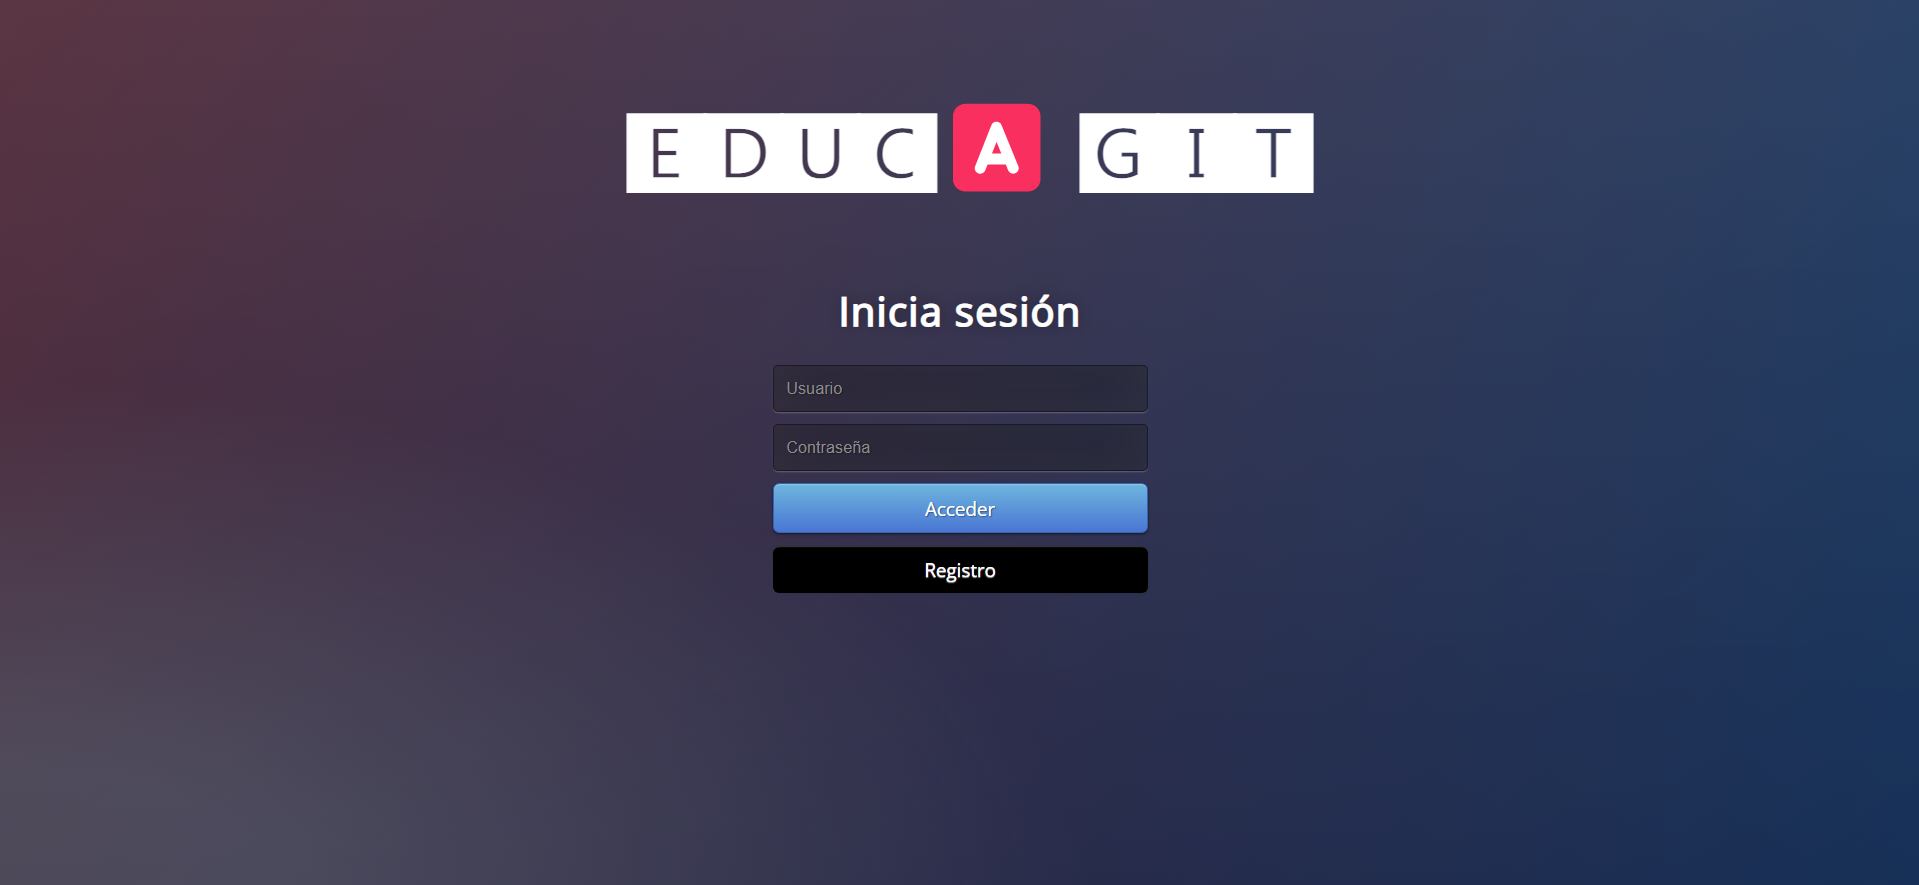
\includegraphics[width=1\textwidth]{incioSesion.png}
  \caption{Vista al no haber iniciado sesión.}
  \label{figure:inicioSesion}
\end{figure}

Una vez situados en esta vista, tenemos dos alternativas, un botón para completar el proceso de registro y por tanto crear una cuenta para el usuario, o en caso de ya haber realizado el proceso de registro iniciar sesión con la cuenta creada. Para ello necesitaremos el nombre de usuario indicado(Como veremos en el proceso de registro este será, el mismo nombre de usuario que disponemos en nuestra cuenta de Github.) y la contraseña indicada en el proceso de registro.


En caso de no estar registrados en la aplicación web, debemos completar dicho procedimiento, para ellos haciendo click en el botón de registro, se nos redirige directamente a la figura~\ref{figure:registro}. En ella debemos completar los siguientes campos, nombre de usuario, como se indica en la web, este debe coincidir con el usuario de Github, un token, el cual a continuación veremos el proceso de obtención, email y contraseña para el registro.

\begin{figure}[h!]
  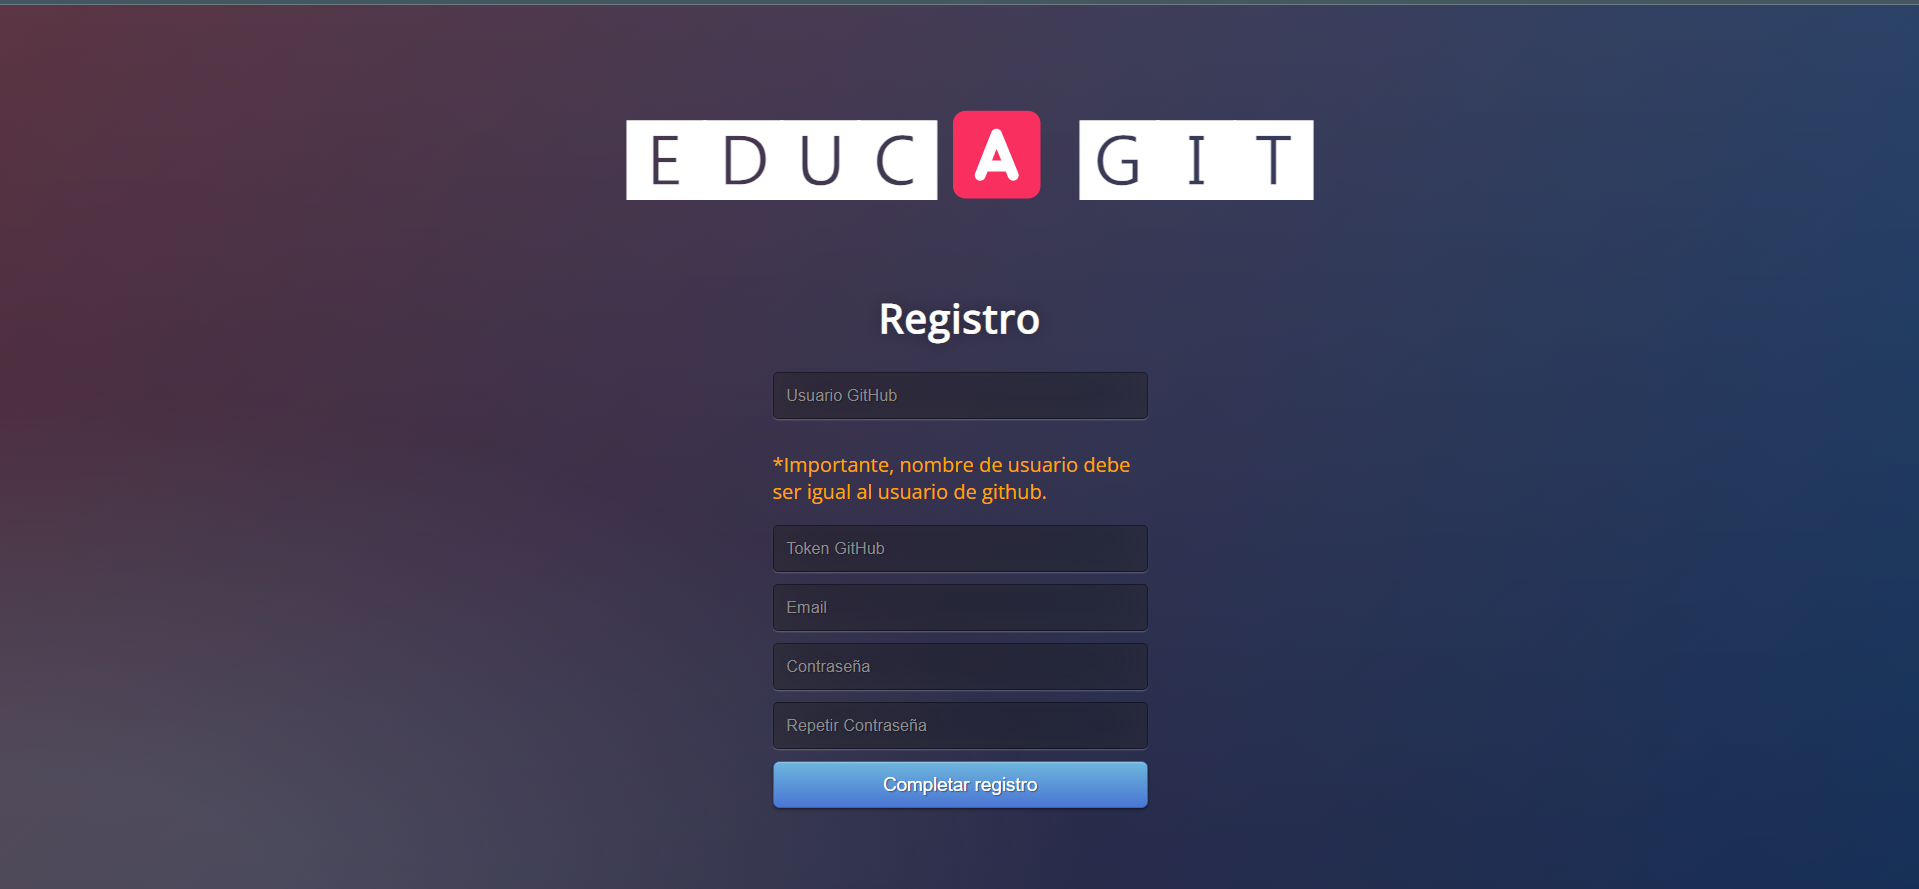
\includegraphics[width=1\textwidth]{registro.png}
  \caption{Formulario de registro.}
  \label{figure:registro}
\end{figure}


\textbf{\href{http://localhost:3000}{\underline{web}}}.


\section{Obtención de un token de GitHub}

En primer lugar debemos acceder a la página oficial de Github\cite{GitHub} y realizar el inicio de sesión con nuestra cuenta de trabajo. Posteriormente accedemos al apartado de configuración como se aprecia en la Figura~\ref{figure:settingsGitHub}.
\begin{figure}[h!]
  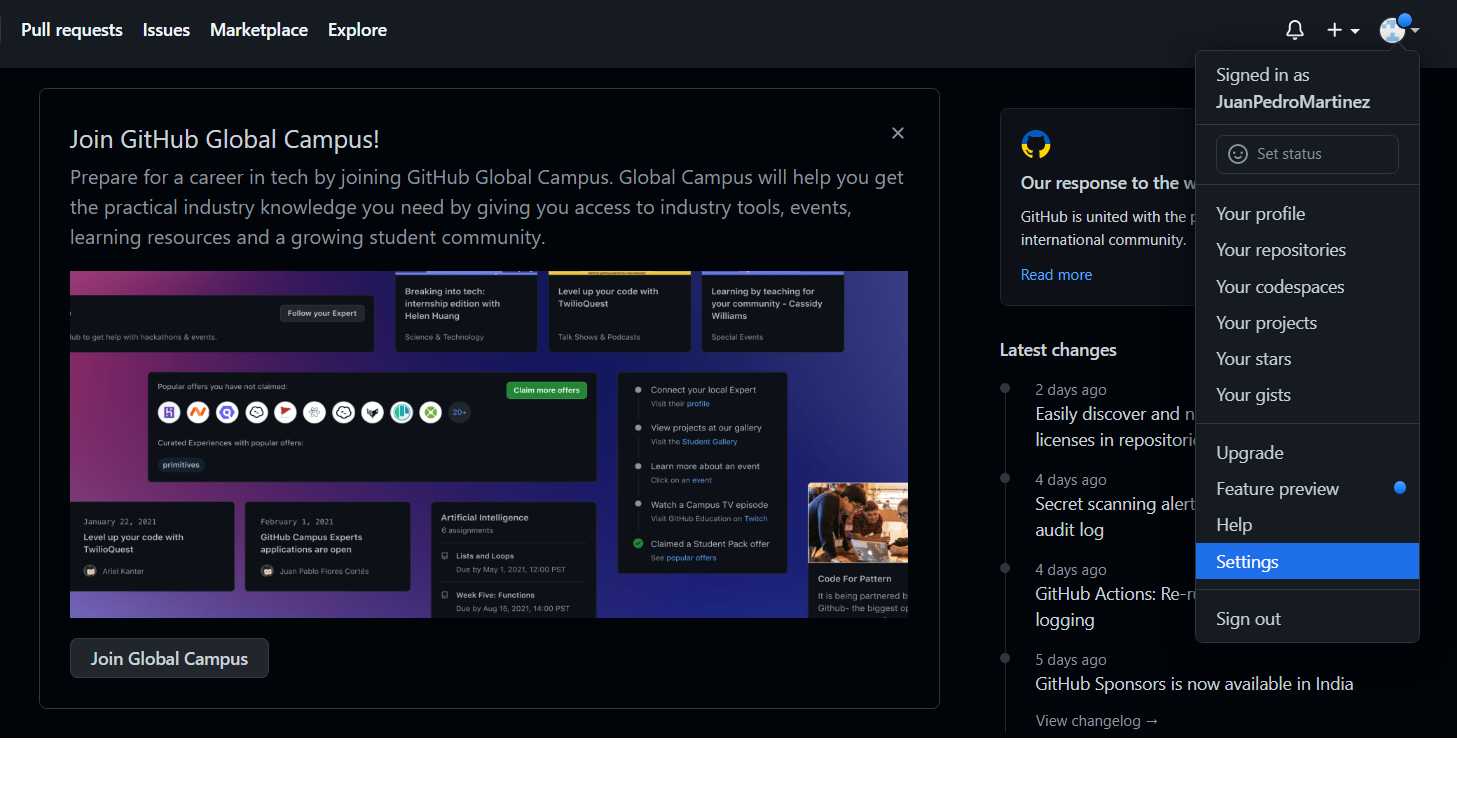
\includegraphics[width=1\textwidth]{githubSettings.png}
  \caption{Acceso a los ajustes en la cuenta de GitHub.}
  \label{figure:settingsGitHub}
\end{figure}

Tras ello, nos llevará a la configuración de la cuenta, donde accederemos mediante el menú del lado izquierdo al submenú configuración de desarrolladores. Figura~\ref{figure:developerSettings}.

\begin{figure}[h!]
  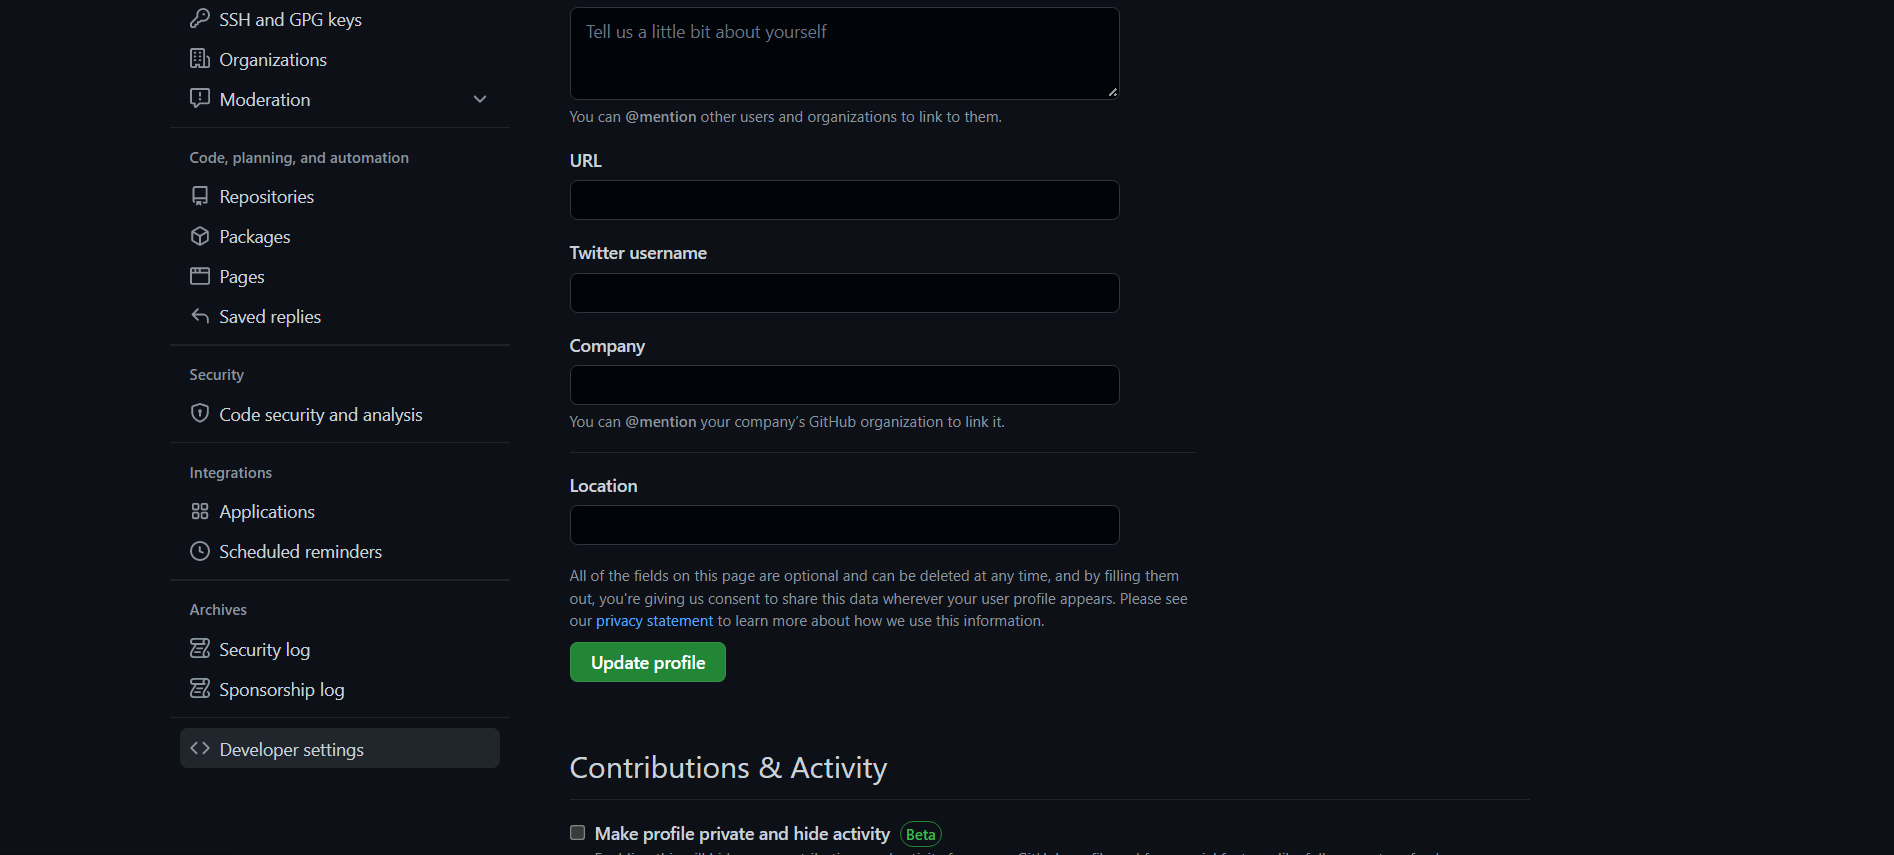
\includegraphics[width=1\textwidth]{githubDeveloperSetting.png}
  \caption{Acceso a los ajusted de desarrollado de GitHub.}
  \label{figure:developerSettings}
\end{figure}

A continuación nos muestra otro menú de apariencia similar en donde seleccionaremos de nuevo en el menú izquierdo el apartado Tokens de acceso personal, y tras ello haremos click generar un nuevo token [Figura~\ref{figure:tokensGitHub}].

\begin{figure}[h!]
  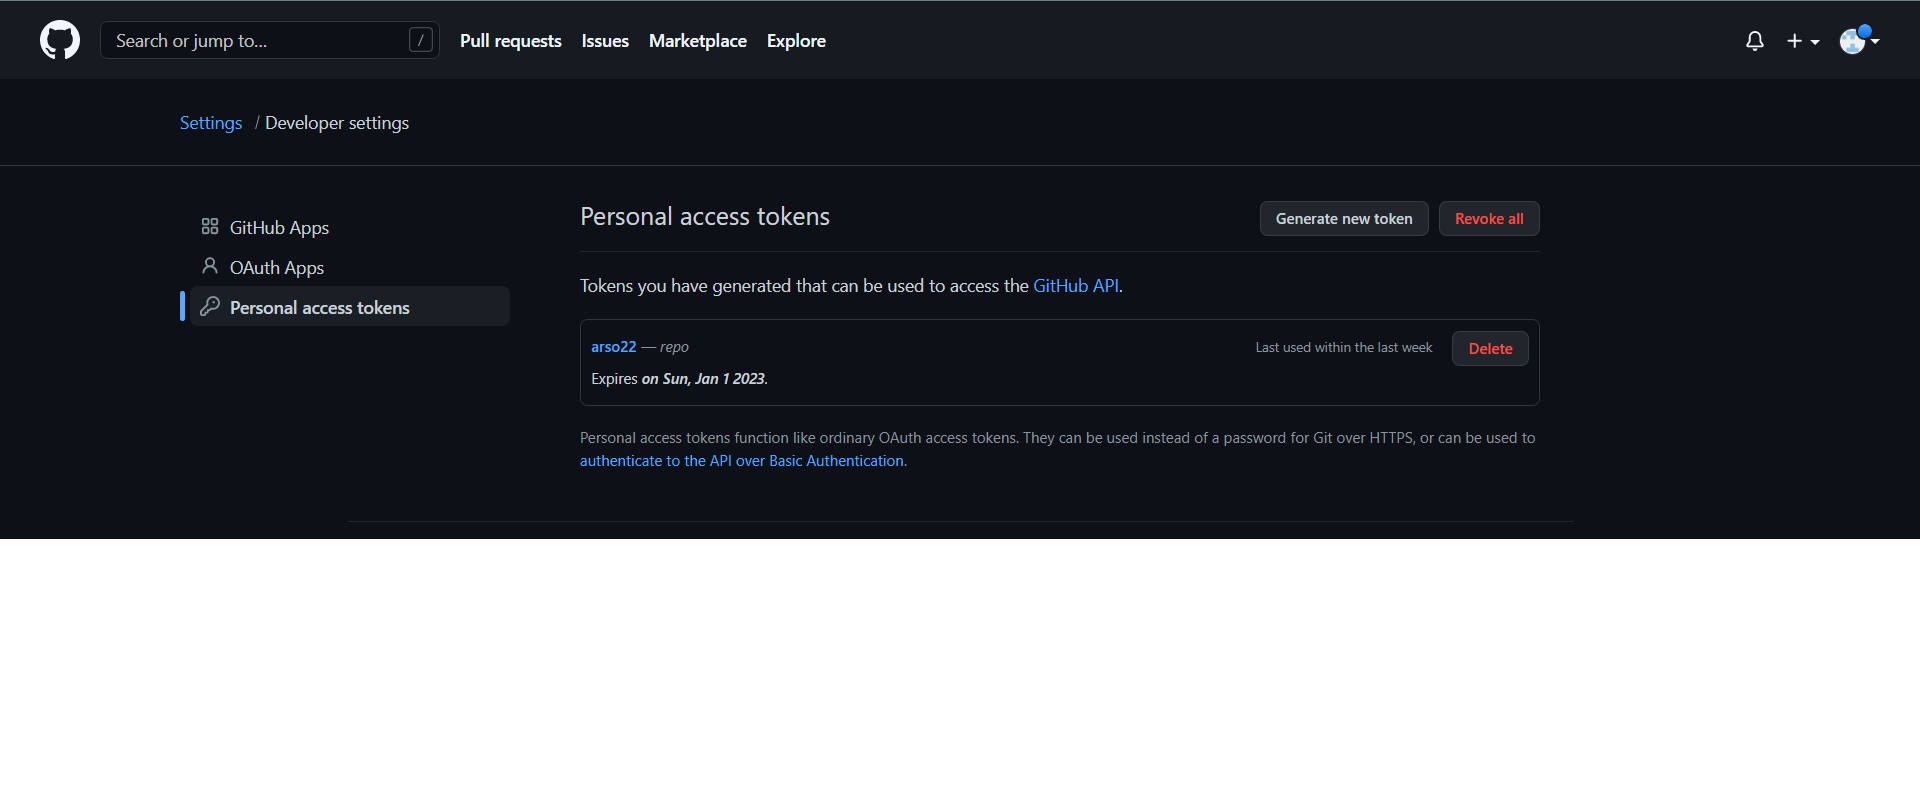
\includegraphics[width=1\textwidth]{accessTokens.png}
  \caption{Acceso al gestor de tokens de GitHub.}
  \label{figure:tokensGitHub}
\end{figure}

Entonces en la nueva vista [Figura~\ref{figure:configToken}] que nos aparece, tendremos múltiples opciones disponibles, las cuales se deben seleccionar en función de los requerimientos de cada tutor.
\begin{figure}[h!]
  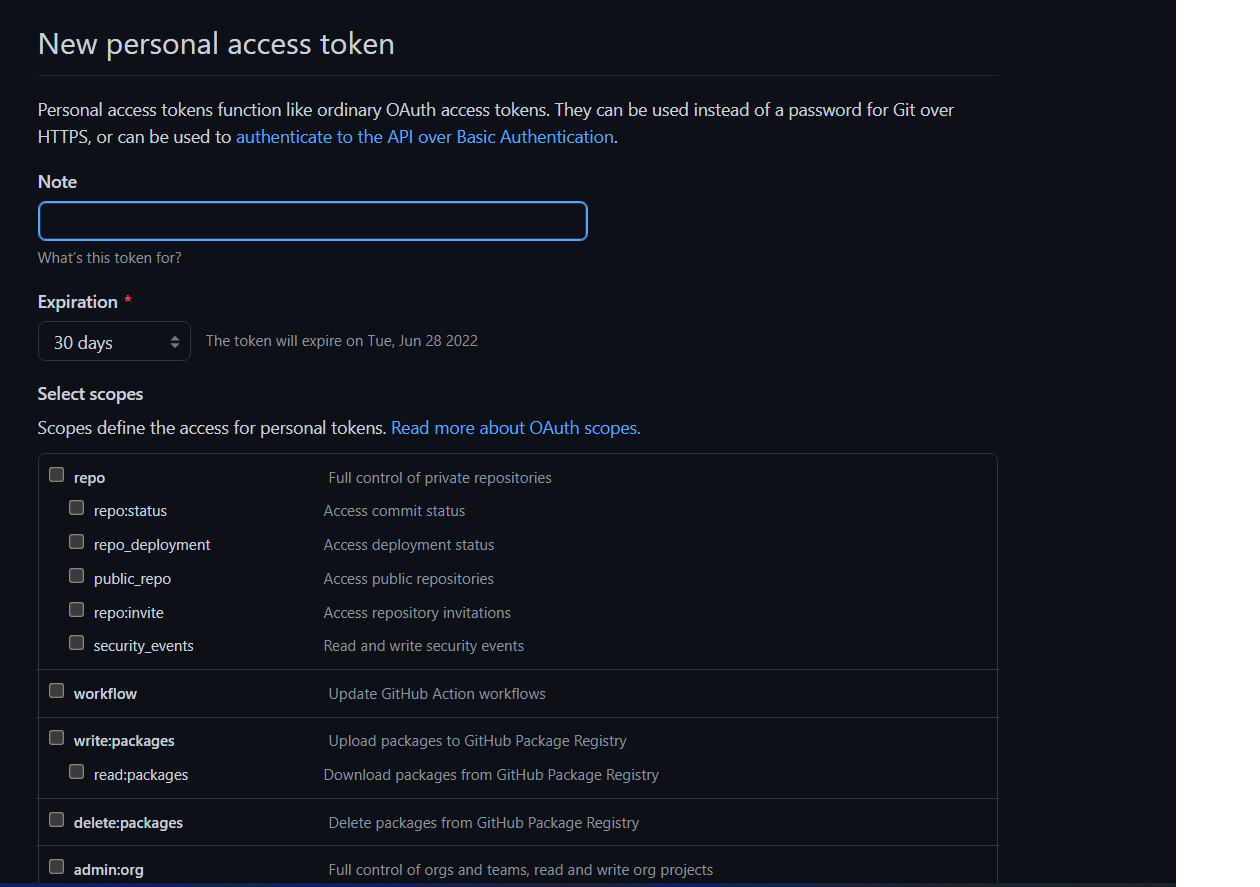
\includegraphics[width=1\textwidth]{newToken.png}
  \caption{Configuración del nuevo token a crear.}
  \label{figure:configToken}
\end{figure}

Encontramos el tiempo de expiración que tendrá el token, dejando de ser válido una vez que este tiempo expire, ofreciendo también la posibilidad de crear un token que no expire. A continuación nos aparecen múltiples seleccionables los cuales indican los privilegios que se otorgan mediante el token, pudiendo seleccionar entre lectura, escritura y modificación de los repositorios asociados a la cuenta. En el caso del proyecto desarrollado únicamente son imprescindibles los permisos de lectura, tanto de repositorios públicos, como privados, como serán normalmente los repositorios de los alumnos.

Una vez seleccionados estas opciones, en la parte inferior encontramos un botón de confirmación para la generación del token y posteriormente se nos mostrará el token, este token consistirá en una cadena de caracteres alfanuméricos, los cuales deberemos conservar como se indica en la página ya que únicamente podremos visualizarlo en el momento de la creación, y teniendo que borrar y crear uno nuevo en caso de pérdida. En cuanto al proyecto, este token se almacena con la información de la cuenta, por lo que una vez añadido ya quedaría funcionando sin necesidad de volverlo a añadir.

Una vez generado el token podremos realizar el proceso de registro, iniciando así sesión en la aplicación, y pudiendo volver a iniciar sesión posteriormente únicamente con el nombre de usuario y contraseña registrados.


Tras el proceso de registro o inicio de sesión, en caso de completarse de manera satisfactoria y correcta, se visualizará la página principal del proyecto, en ella debemos observar los repositorios de nuestra cuenta de Github y repositorios en los cuales participamos como colaborador, esta información se verá reflejada en la tabla de la figura X.
En caso de no visualizar los repositorios, es probable que haya habido algún problema en el proceso de creación del token y deberá repetirse.

En la página principal, Figura~\ref{figure:mainPage}, observamos una interfaz simple mediante la cual podemos implementar la funcionalidad previamente explicada. En primer lugar, encontramos los repositorios asociados a nuestra cuenta, obteniendo la información a modo de tabla del nombre de cada repositorio y su correspondiente creador. Además encontramos, una celda, con múltiples botones mediante los cuales podemos, ir directamente a la página de GitHub del repositorio correspondiente, copiar la url del repositorio  o un botón que como más adelante explicaremos, sirve para añadir un repositorio a alguna asignatura creada.

\begin{figure}[h!]
  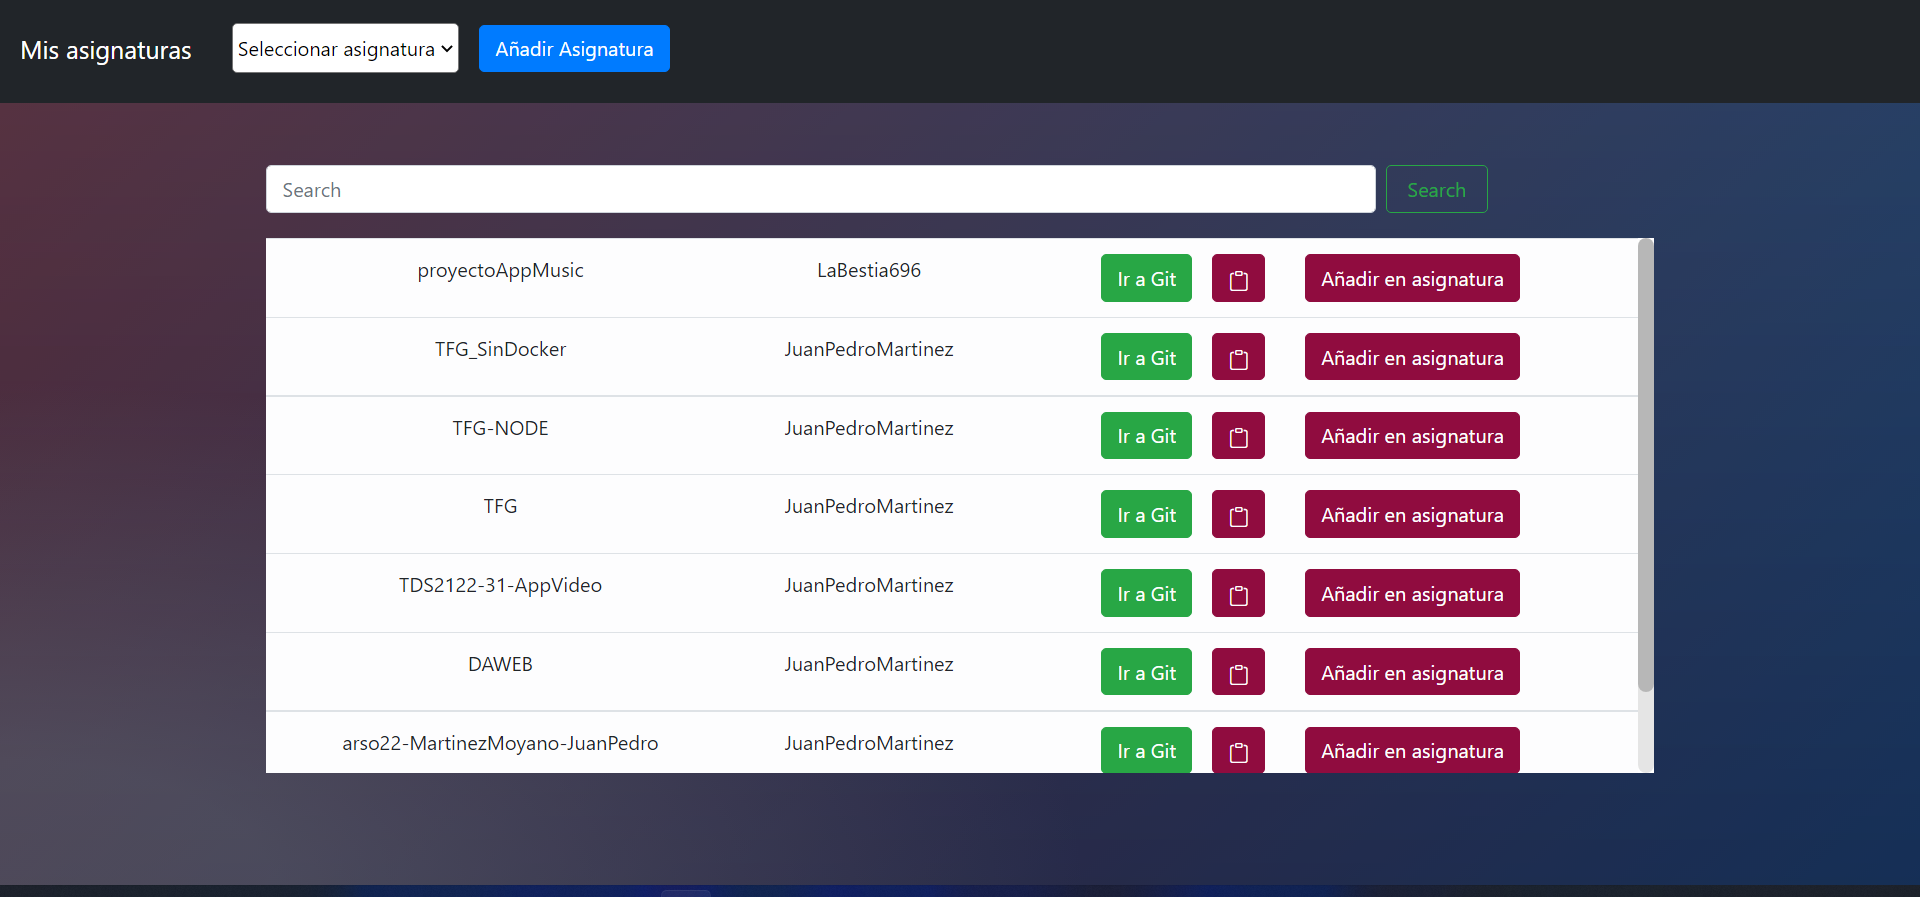
\includegraphics[width=1\textwidth]{paginaPrincipal.png}
  \caption{Página principal, tras realizar login o registro.}
  \label{figure:mainPage}
\end{figure}

También encontramos una barra de búsqueda, con la que podremos introducir una cadena con la que se filtraran los repositorios mostrados, haciendo así más sencillo encontrar un determinado repositorio.

En la parte superior, también encontramos un selector, con el cual podremos acceder a alguna de las asignaturas creadas Figura~\ref{figure:mainPageSeleccion}.
\begin{figure}[h!]
  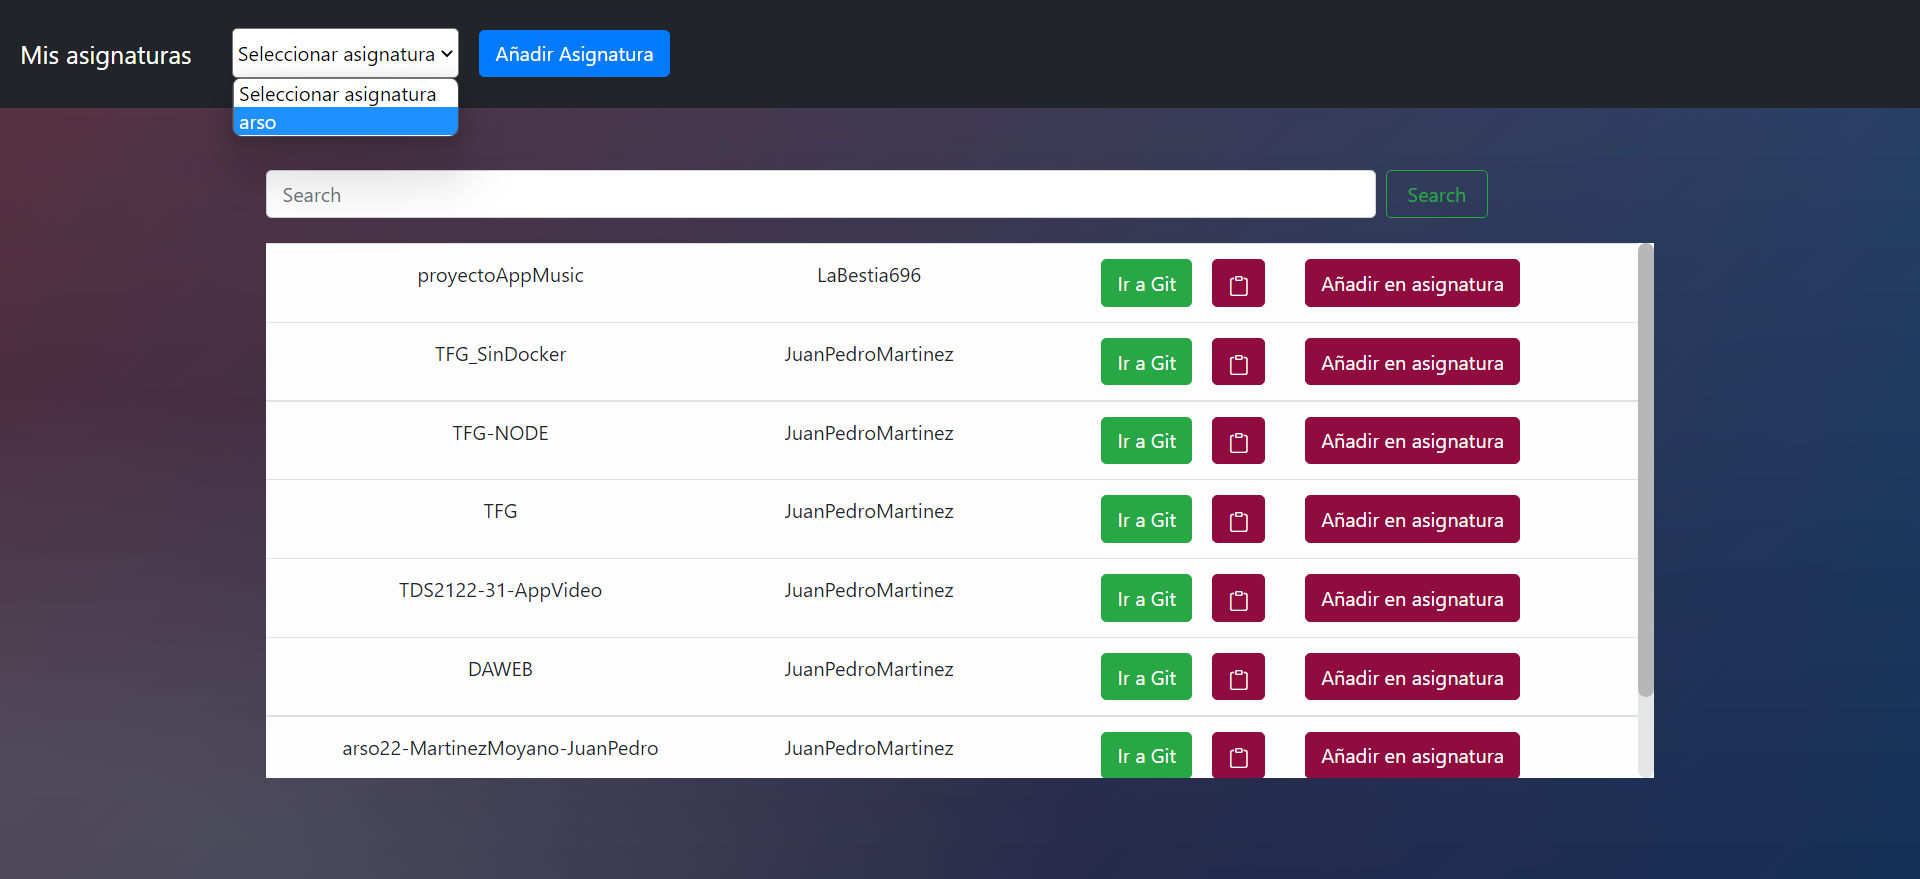
\includegraphics[width=1\textwidth]{seleccionAsignatura.png}
  \caption{Selección de una asignatura en la página principal.}
  \label{figure:mainPageSeleccion}
\end{figure}


\section{Proceso de creación de asignaturas}

    La aplicación, como hemos visto a lo largo de la memoria del proyecto, permite crear la entidad asignatura, mediante la cual, se pueden gestionar los repositorios correspondientes, para ello, cada asignatura tiene el nombre como tál y una cadena de coincidencias con el nombre del repositorio, es decir, como vimos en los requisitos de la aplicación, un tutor específica a sus alumnos que deben crear el repositorio introduciendo en dicho nombre la cadena de texto nombreAsignatura-Curso, con esto, posteriormente el tutor crea en la aplicación una asignatura asignándole el nombre correspondiente y indicando en la entrada de texto de la figura X, cadena de coincidencias con el valor anunciado a los alumnos (nombreAsignatura-Curso), en la página principal hacemos click en la parte superior en el botón de añadir asignatura, nos muestra una ventana emergente como en la figura~\ref{figure:addAsignatura}.

    \begin{figure}[h!]
      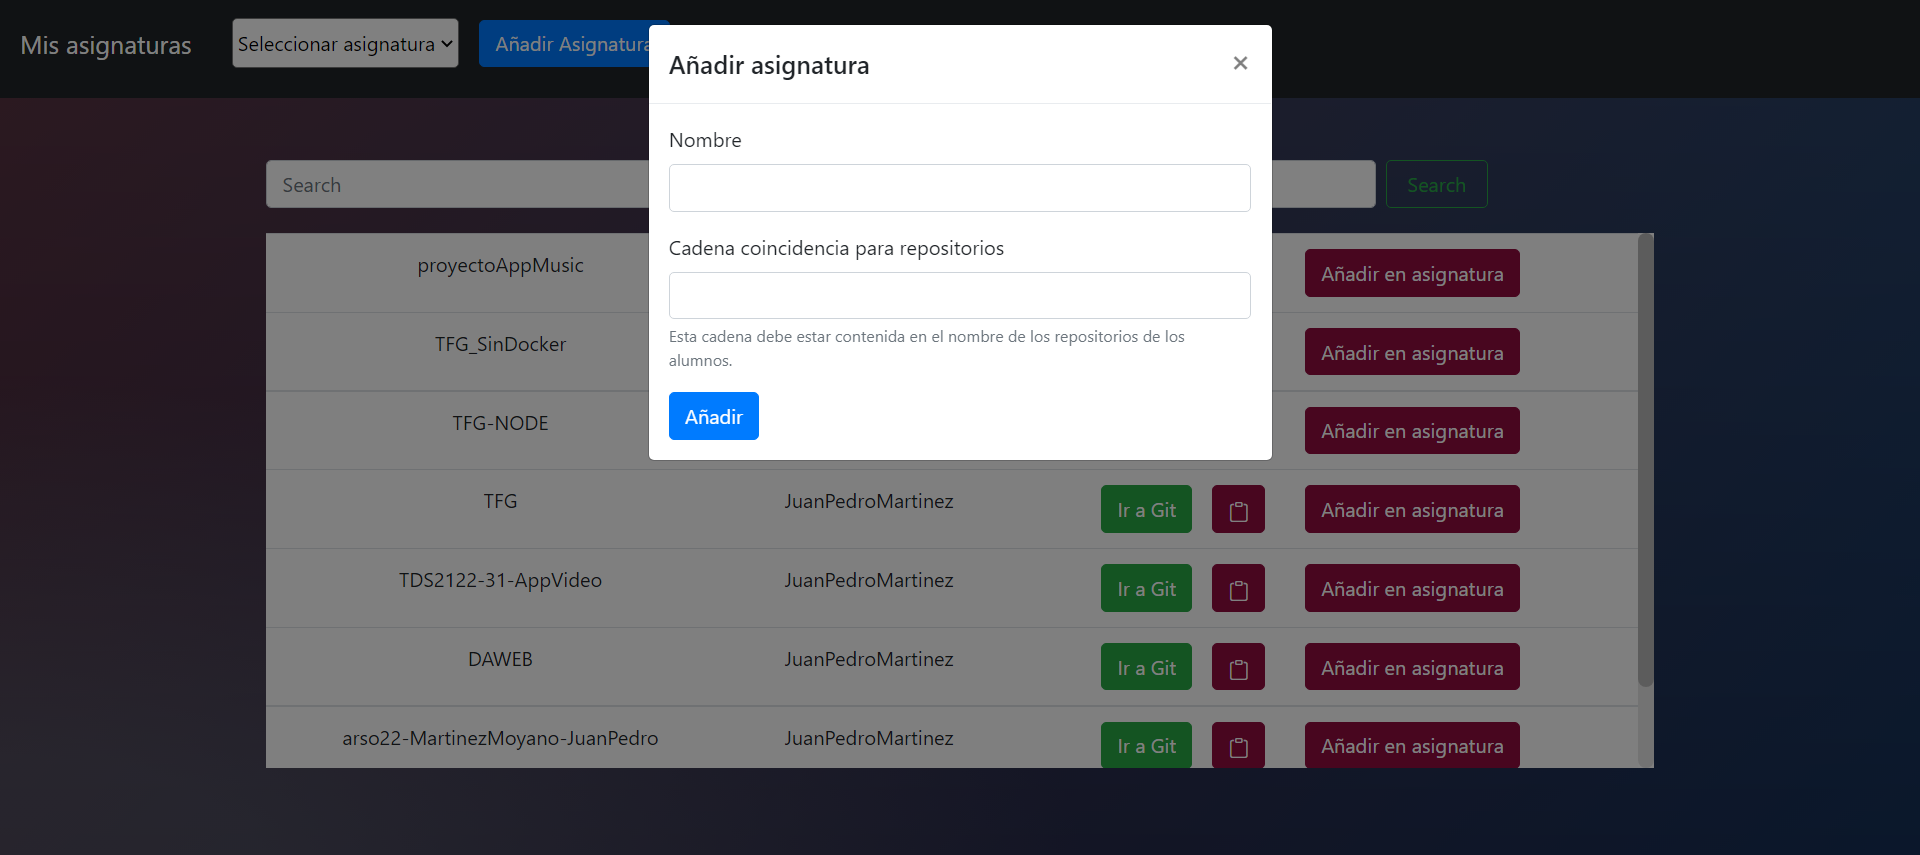
\includegraphics[width=1\textwidth]{addAsignatura.png}
      \caption{Ventana modal para añadir asignatura.}
      \label{figure:addAsignatura}
    \end{figure}

    De esta forma al seleccionar la asignatura en el selector de la parte superior, se filtran automáticamente los repositorios de dicha asignatura, haciendo mucho más sencilla la gestión de los repositorios de asignaturas y cursos. Figura~\ref{figure:filtradoAsignatura}.

    \begin{figure}[h!]
      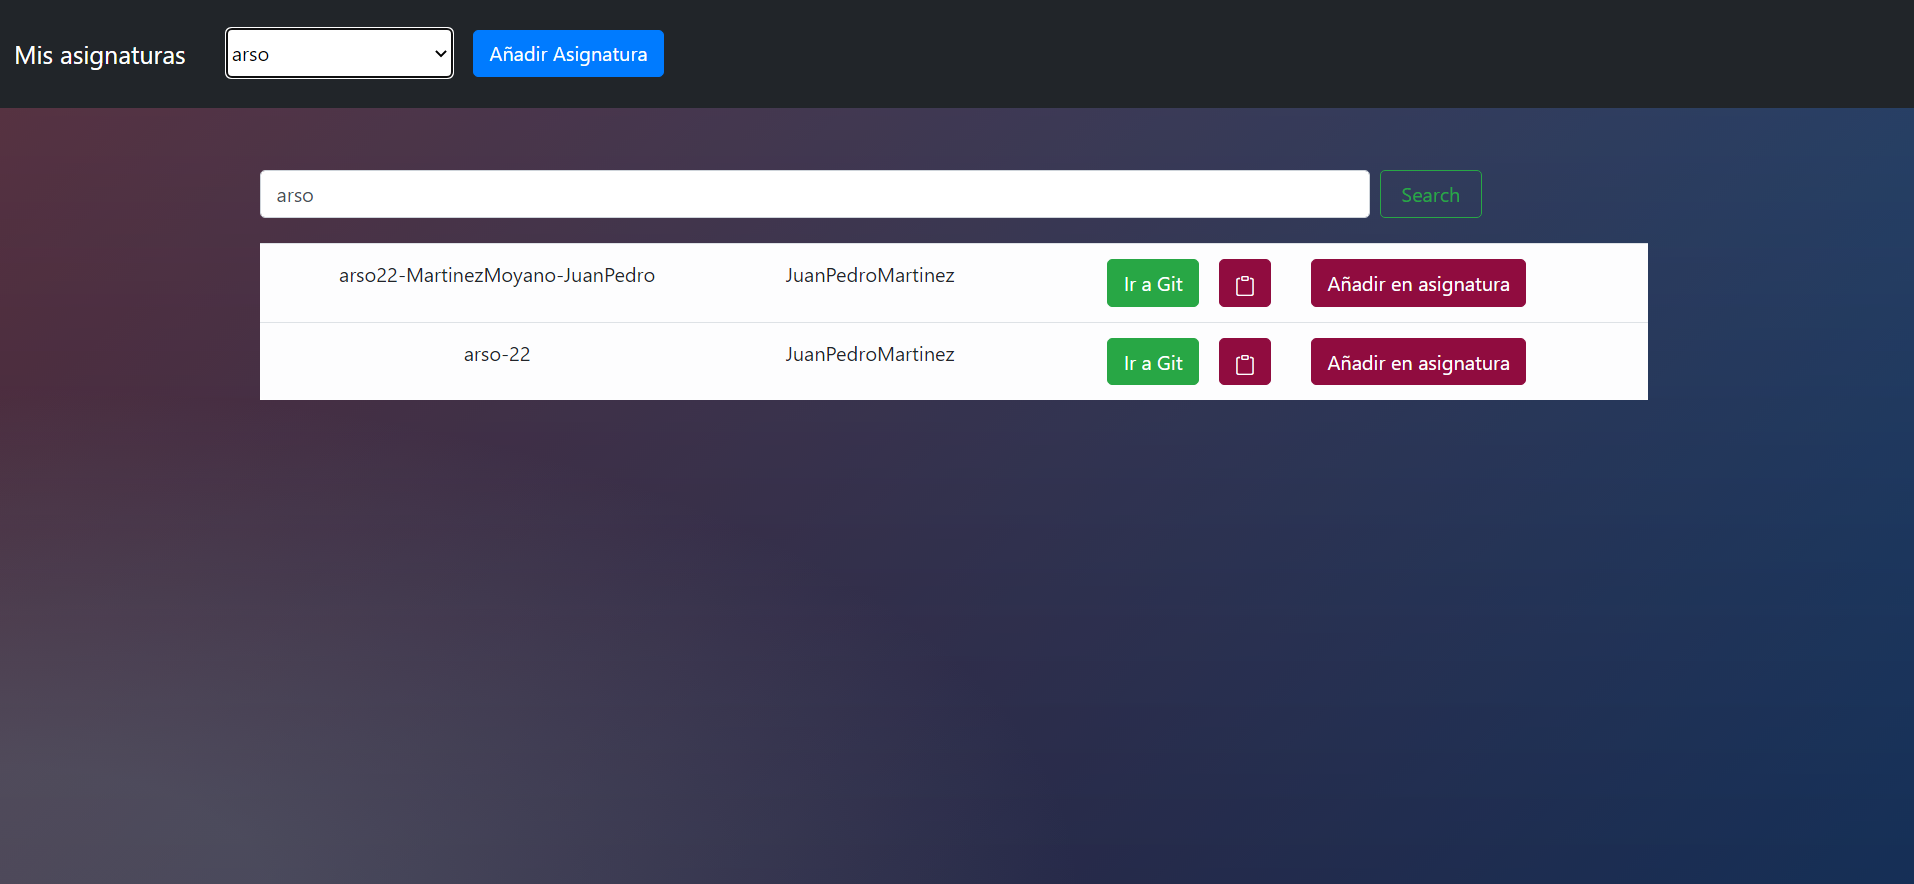
\includegraphics[width=1\textwidth]{filtradoPorAsignatura.png}
      \caption{Ejemplo de filtrado por asignatura ARSO.}
      \label{figure:filtradoAsignatura}
    \end{figure}
    En algunos casos, es posible que ocurra que algún alumno no realice correctamente la creación del repositorio con la cadena de coincidencias indicada por el tutor, en este caso, se ofrece la posibilidad de añadir un repositorio a una asignatura de forma manual. Como vemos a continuación.




\section{Adición manual de un repostorio en una asignatura}


    Previamente a este paso, la asignatura debe haber sido correctamente creada.
    Para añadir un repositorio a una asignatura, en primer lugar debemos encontrar el repositorio que se desea añadir, buscándolo de forma manual o utilizando la barra de búsqueda de la página principal, una vez encontrado el repositorio, hacemos click en el botón “añadir en asignatura”, apareciéndose una ventana emergente, correspondiente a la figura~\ref{figure:repoAAsignatura}

    \begin{figure}[h!]
      \includegraphics[width=1\textwidth]{AñadirAsignaturaRepositorio.png}
      \caption{Ventana modal añadir repositorio a asignatura.}
      \label{figure:repoAAsignatura}
    \end{figure}

    En esta ventana, seleccionamos la asignatura con el selector sobre la que queremos añadir el repositorio y hacemos click en el botón de confirmación añadir. 

    Una vez realizado este paso, el repositorio se añadirá a la asignatura mostrando posteriormente al seleccionar las asignaturas con el selector de la página principal, y quedando persistentes para la misma.

    En la figura~\ref{figure:asignaturaConReposManuales}, vemos un ejemplo de adición de un repositorio a una asignatura, en este caso se ha añadido el repositorio TFG sobre la asignatura arso, de tal forma que al seleccionar arso en el selector de la página principal, muestra tanto los repositorios que coinciden con la cadena de coincidencias de la asignatura, como los repositorios añadidos de forma manual.

    \begin{figure}[h!]
      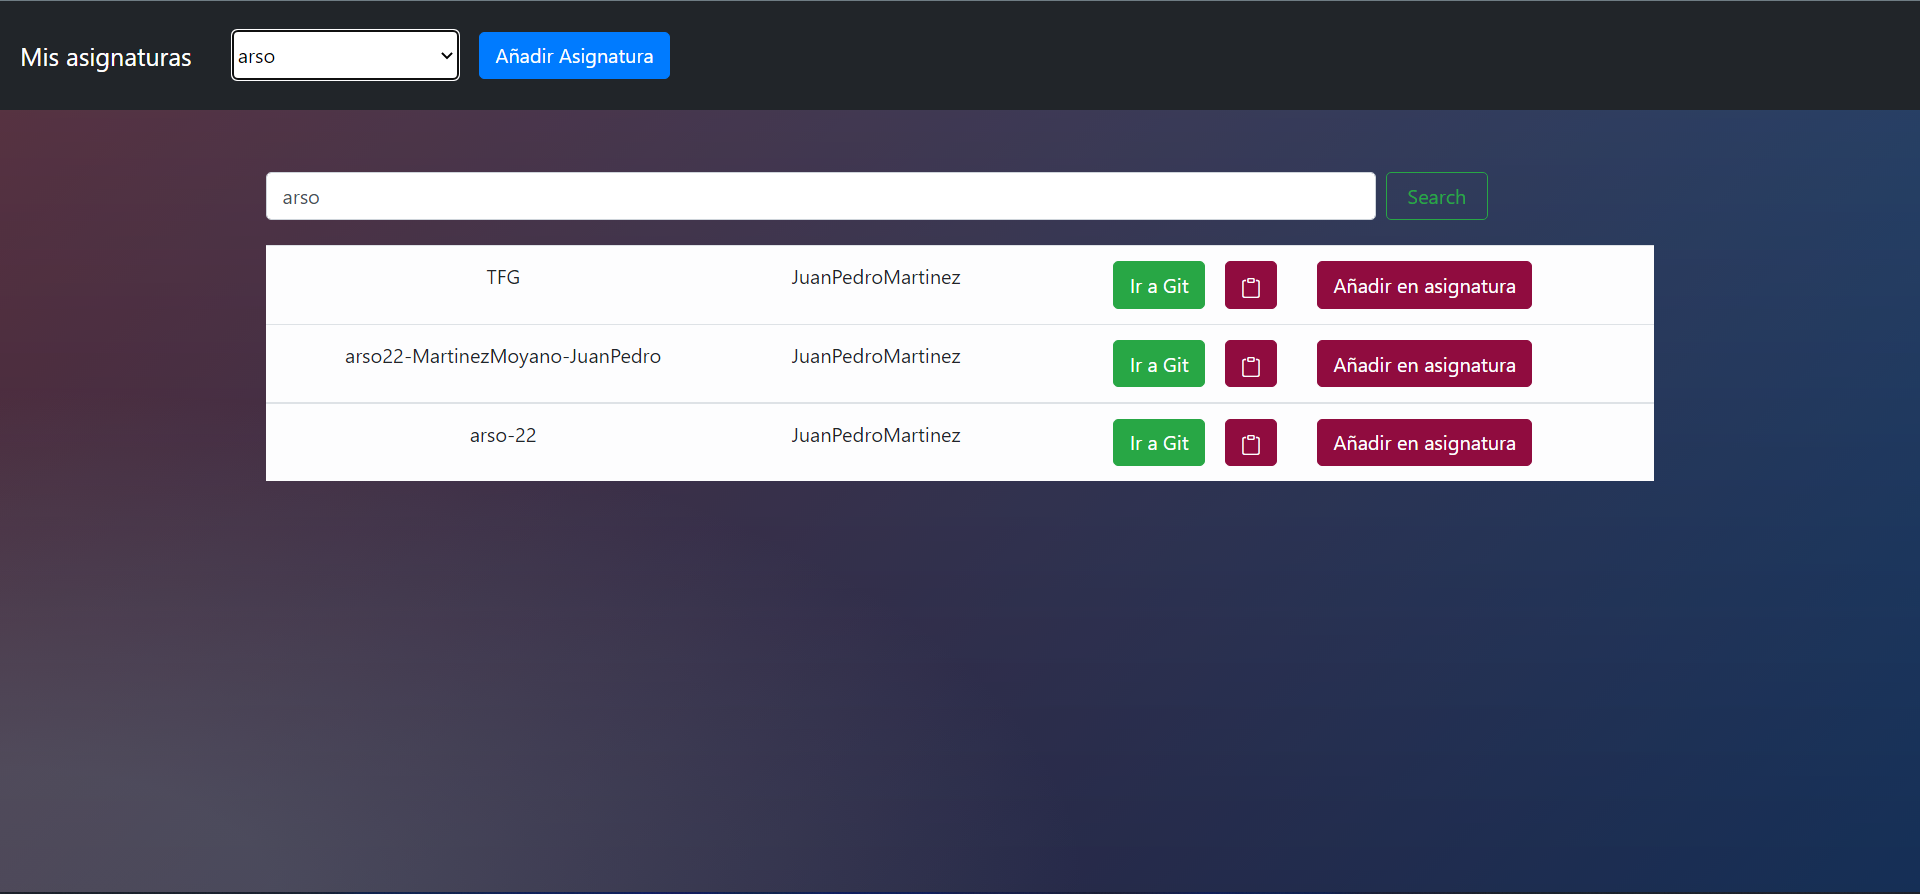
\includegraphics[width=1\textwidth]{repositorioAdicionadoEnAsignatura.png}
      \caption{Ejemplo asignatura con repositorios manualmente añadidos.}
      \label{figure:asignaturaConReposManuales}
    \end{figure}

\section{Acceso al panel de estadísticas de un repositorio}

    Sobre la página principal, en la tabla de repositorios, en cualquier momento,haciendo click en el interior de la fila de la tabla correspondiente al repositorio, accederemos al panel de estadísticas del mismo. De tal forma que veremos una nueva interfaz, correspondiente a la figura~\ref{figure:estadRepo}.

    \begin{figure}[h!]
      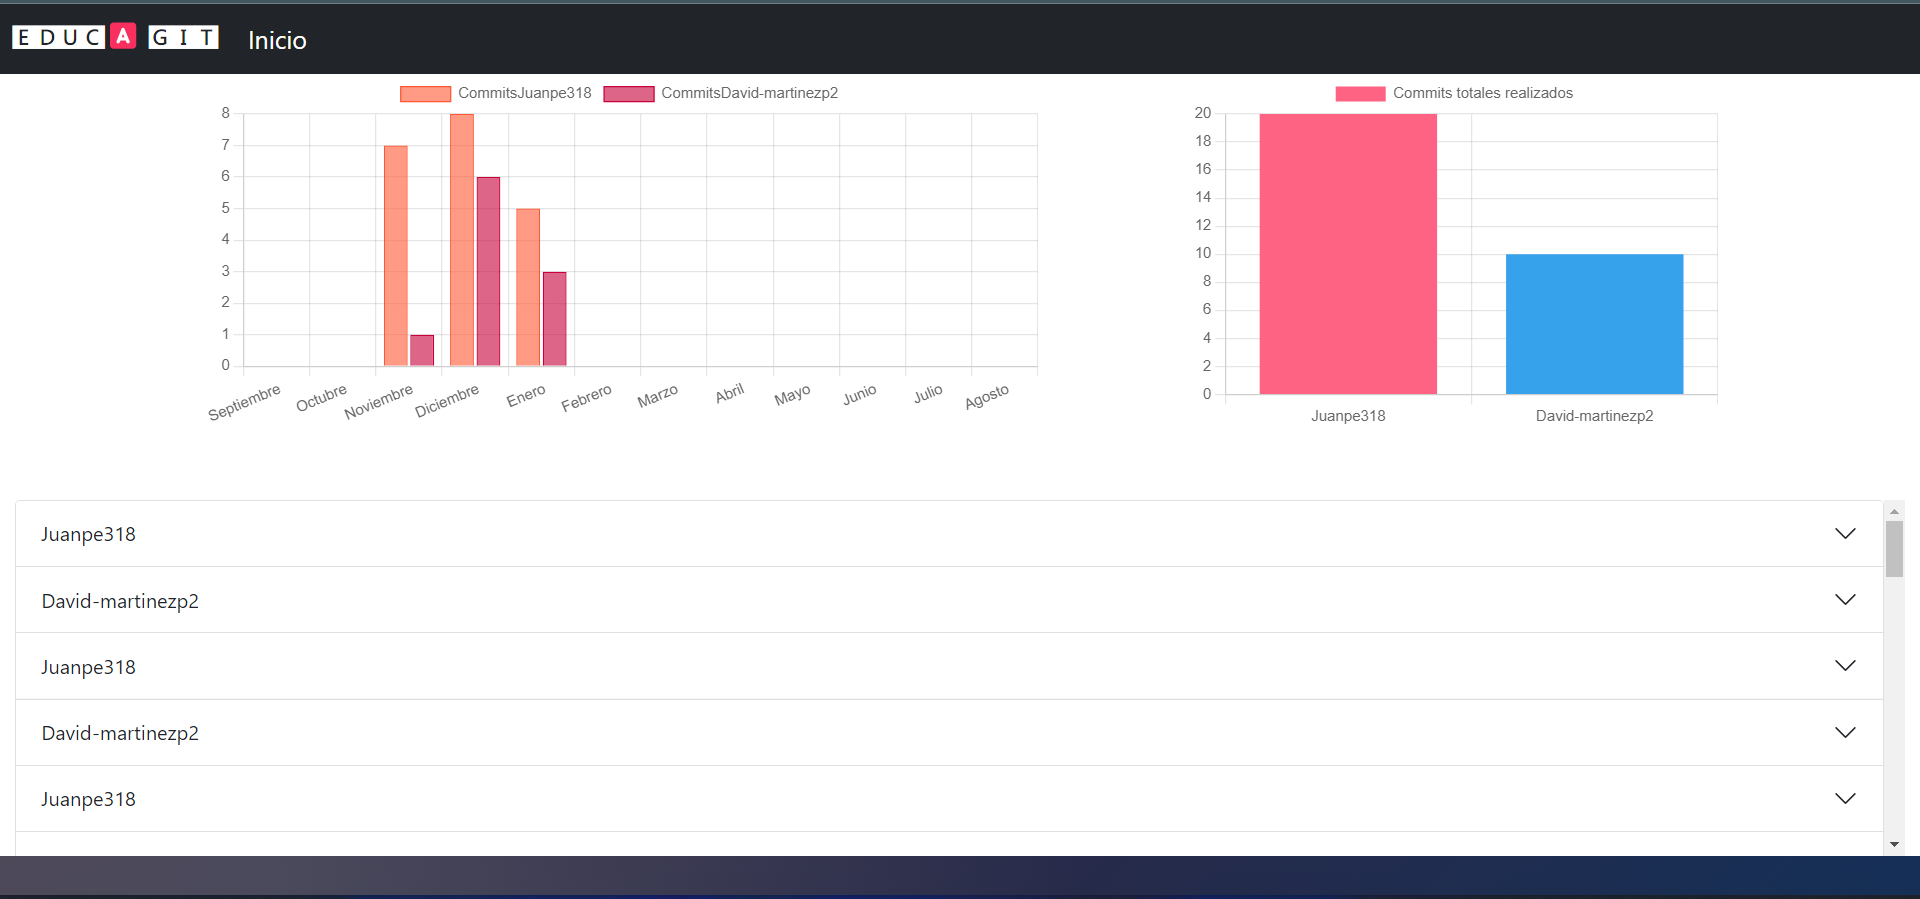
\includegraphics[width=1\textwidth]{estadisticasRepositorio.png}
      \caption{Interfaz del panel de estadísticas de un repositorio.}
      \label{figure:estadRepo}
    \end{figure}

    En ella encontramos los siguientes elementos,
    \begin{enumerate}
      \item Un primer gráfico, en el lado izquierdo el cual nos muestra la distribución de commits de cada uno de los colaboradores del repositorio a lo largo del curso educativo. Pudiendo conocer el número de commits mensuales de cada alumno y visualizar un gráfico representativo de dichos datos.
      \item Un segundo gráfico, en el lado derecho el cual muestra el número de commits totales realizados sobre un repositorio. Especialmente útil cuando queremos averiguar si existen sobrecargas de trabajo entre diferentes alumnos.
      \item Por último en la parte inferior de los gráficos encontramos desplegables los cuales muestran cada uno de los commits realizados sobre el repositorio, de tal forma que los últimos commits aparecen al principio y los primeros al final. Para cada commit, se muestra el autor del commit, y al hacer click sobre el desplegable, se nos muestra de forma textual los cambios que se han realizado en dicho commit, pudiendo así ver que tan grandes son las modificaciones que han implicado dicho commit. Figura~\ref{figure:imagenPatch}.
    \end{enumerate}

    \begin{figure}[h!]
      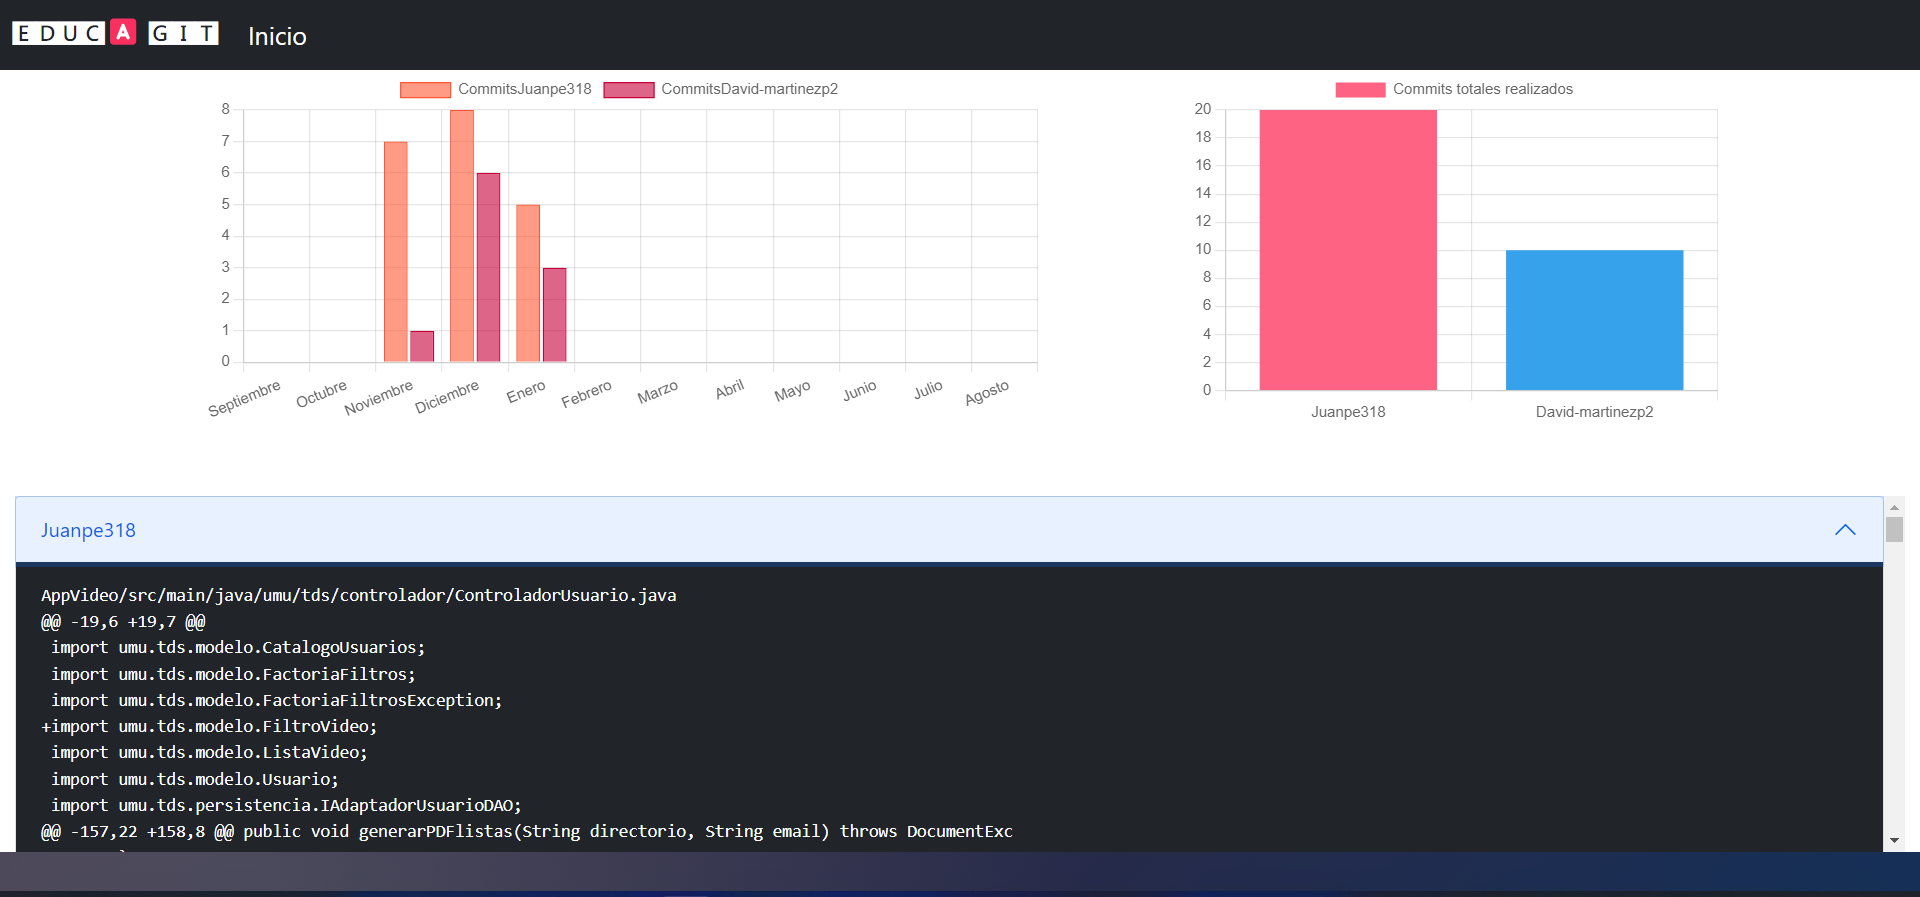
\includegraphics[width=1\textwidth]{analisisPatchRepositorio.png}
      \caption{Desplegables de la parte inferior del panel de estadísticas.}
      \label{figure:imagenPatch}
    \end{figure}

\chapter{Estructura del proyecto y puesta en marcha.\label{09EstructuraYpuesta}}

El proyecto, está publicado en GitHub sobre el siguiente \textbf{\href{https://github.com/JuanPedroMartinez/TFG-NODE}{\underline{enlace}}} quedando la estructura del proyecto dividida en los siguientes directorios y ficheros.

\begin{itemize}
  \item En primer lugar, encontramos la carpeta memoria, en la cual esta implementada toda la lógica del lenguaje LATEX para la generación de este fichero .pdf
  
  \item En segundo lugar, el directorio modules, contiene módulos propios desarrollados en javascript, para el manejo de la entidad asignatura y su persistencia.
  
  \item Por otra parte, encontramos una carpeta restjs, correspondiente al segundo servidor, encargado de gestionar las peticiones al API REST de GitHub, en este directorio, al igual que en el raíz, encontraremos un fichero package.json y app.js los cuales corresponden al paquete de dependencias del proyecto y la aplicación principal para Node.js.
  
  \item En el directorio scripts, tenemos ubicado el script correspondiente para la inicialización de una base de datos MySQL, cumpliendo los requerimientos y tablas necesarios para el funcionamiento de la aplicación.
  
  \item En la carpeta static, encontramos los ficheros estáticos, es decir, los ficheros css y javascript usados y solicitados por el navegador del cliente.
\end{itemize}

Además, en el proyecto encontramos dos ficheros ``Dockerfile'', uno en la carpeta raíz y otro situado dentro de la carpeta del segundo servidor ``restjs''. Estos se encargan de construir las imágenes de los contenedores, en los cuales se correrán los servicios Node.js.

Por otra parte, en el directorio raíz encontramos el fichero docker-compose.yml'', este fichero se corresponde con el fichero de configuración de docker compose, el cual nos permitirá lanzar el proyecto de manera totalmente automática y sobre cualquier plataforma. En este fichero se realiza la configuración necesaria para la puesta en marcha de los dos servidores Node.js y la base de datos MySQL, configurando además una red interna, sobre la cual se intercomunican los servicios creados.

En cuanto el despliegue del proyecto, necesitamos tener Docker instalado en el sistema, e iniciar Docker, en el caso de trabajar sobre un sistema operativo Windows, abrimos la aplicación ``Docker-Desktop''\cite{DockerDesktop}, o en caso de estar bajo un sistema UNIX, podemos ejecutar el comando ``\emph{sudo systemctl start docker}''.

Una vez iniciado el docker, únicamente debemos acceder a la carpeta del proyecto mediante una consola, e introducir el comando ``\emph{docker compose up}''.
Este comando construirá las imágenes docker de los servicios creados, obteniendo además las imágenes de Node.js y MySQL, llevando a cabo la configuración de todos los servicios y la puesta en marcha de todos ellos.

Tras esperar que el proceso se inicie y los servidores queden escuchando, y la base de datos esté lista para recibir conexiones, el proyecto estará completamente desplegado y funcionando.


  

%%% Local variables:
%%% TeX-master: "memoria.tex"
%%% coding: utf-8
%%% ispell-local-dictionary: "spanish"
%%% TeX-parse-self: t
%%% TeX-auto-save: t
%%% fill-column: 75
%%% End:
